\chapter{Experiments}

In this chapter, We present the results of experiments which we carried out to verify the hybrid and q-learning algorithm approaches ,the antipatterns  implementation, the fitness objective function and the metaheuristics used by the testbed tool.   Six experiments were conducted to validate the proposed approach. The first experiment was performed on an emulated component. The second and third experiments are conducted in an testbed developed appplication. The fourth  experiment was performed using an installed Moodle application. The fifth and sixth experiments are performned using an installed JPetStore application.

\section{Emulated Class Test Experiment}


The first experiment aimed to perform performance, load, and stress testing on a simulated component. The purpose of using a simulated component was to be able to perform a greater number of generations in a shorter time available and eliminate variables such as the use of databases and application servers. The first experiment used a test class  named SimulateConcurrentAccess. This class has a static variable named \textit{x} and a set of methods that use the variable in a synchronized context ( Listing \ref{classsimulated}). The experiment was executed using the JMeter Java Request Sampler Component with IAdapter.

\lstdefinestyle{outline}{
		language=Java,
         basicstyle=\scriptsize\ttfamily,
         numberstyle=\tiny,
         numbersep=5pt,
         tabsize=2,
         extendedchars=true,
         breaklines=true,
         keywordstyle=\color{black}\bf,
         frame=b,  % <<<<<<<<<<<<<<<<<<<<<<<<<<
         stringstyle=\color{green!40!black}\ttfamily,
         showspaces=false,
         showtabs=false,
         numbers=left,
         xleftmargin=17pt,
         framexleftmargin=17pt,
         framextopmargin=1pt, % <<<<<<<<<<<<<<<<<<<<<<
         showstringspaces=false,
         %backgroundcolor=\color[RGB]{200,200,200},
         belowcaptionskip=0pt
}

\begin{lstlisting}[style=outline,caption={SimulateConcurrentAccess class},float,label=classsimulated]
public class SimulateConcurrentAccess {
  @Test
  public void firstScenario() {		
    synchronized (StaticClass.class) {
			for (int i = 0; i <= 1000; i++) {
				StaticClass.x += i;
			}
			StaticClass.x = 0;
		}
	}
	
	  @Test
  public void secondScenario() {		
    synchronized (StaticClass.class) {
			for (int i = 0; i <= 2000; i++) {
				StaticClass.x += i;
			}
			StaticClass.x = 0;
		}
	}
\end{lstlisting}


The experiment used the following fitness function:

\begin{equation}
\begin{aligned}
fitness=0.9* 90percentiletime\\
+0.1*80percentiletime\\+
0.1*70percentiletime+\\
0.1*maxResponseTime+\\
0.2*numberOfUsers-penalty
\end{aligned}
\end{equation}

This fitness function is the same function represented in the section VII with the manually adjustable user-defined weights filled out. This fitness function intended to find individuals with the highest percentile of 90\%, followed by individuals with a higher percentile time of 80\% and 70\%, maximum response time, and number of users.

The first experiment ran for 27 generations, and the second experiment  performed 6 generations, with 300 executions by generation (100 times for each algorithm),  generating 300 new individuals. The experiments used an initial population of 100 individuals. The genetic algorithm used the top 10 individuals from each generation in the crossover operation. The Tabu list was configured with the size of 10 individuals and expired every 2 generations.  The mutation operation was applied to 10\% of the population on each generation. 

Fig.\ref{fig:exp1bestresults} presents the best results in 27 generations applied in the first experiment. The figure shows the results obtained with the algorithms with and without collaboration. The $x$ axis  represents the generation number, and the $y$ axis represents the best fitness value obtained until the current generation.
A higher value in the figure means that the scenario has a greater response time by the application under test. The results of the experiment showed that the use of cooperation between the three algorithms resulted in finding the individuals with better fitness values.

\begin{figure}[h]
\centering
\caption{Best results obtained in 27 generations}
\includegraphics[width=1\textwidth]{./images/generationcomparative.png}
\label{fig:exp1bestresults}
\end{figure}

Table \ref{tab:averagefirst} presents the results obtained by the hybrid metaheuristic (HM) approach, genetic algorithm (GA), simulated annealing (SA), and Tabu search (TS) from 27 generations in the first experiment. The values are the maximum fitness value obtained by each algorithm. 

\begin{table}[h]
\centering
\caption{Maximum value of the fitness function by algorithm}
\label{tab:averagefirst}
\begin{tabular}{|l|l|l|l|l|}
\hline
GEN & HM & TS  & GA    & SA    \\ \hline
1          & 11238 & 11238         & 11238 & 11238 \\ \hline
2          & 11804 & 11596         & 11801 & 10677 \\ \hline
3          & 11787 & 8932          & 8411  & 10869 \\ \hline
4          & 11723 & 9753          & 9611  & 10760 \\ \hline
5          & 8164  & 9780          & 10738 & 4794  \\ \hline
6          & 11802 & 9781          & 11086 & 6120  \\ \hline
7          & 9985  & 5782          & 11272 & 11798 \\ \hline
8          & 11803 & 11749         & 10084 & 11309 \\ \hline
9          & 11806 & 7284          & 11633 & 10766 \\ \hline
10         & 11807 & 9386          & 11717 & 4557  \\ \hline
11         & 11802 & 9653          & 11802 & 11151 \\ \hline
12         & 11807 & 10594         & 11793 & 9434  \\ \hline
13         & 11802 & 10848         & 10382 & 11805 \\ \hline
14         & 11801 & 11551         & 7219  & 10237 \\ \hline
15         & 11807 & 1701          & 7189  & 9338  \\ \hline
16         & 11813 & 6203          & 11758 & 5321  \\ \hline
17         & 11805 & 10720         & 10805 & 11748 \\ \hline
18         & 9600  & 6371          & 11698 & 7818  \\ \hline
19         & 11733 & 8160          & 11648 & 11509 \\ \hline
20         & 9589  & 9428          & 11805 & 4813  \\ \hline
21         & 11800 & 9463          & 11798 & 10801 \\ \hline
22         & 11805 & 11799         & 11804 & 6029  \\ \hline
23         & 11836 & 11655         & 11800 & 3579  \\ \hline
24         & 11805 & 11512         & 11803 & 5761  \\ \hline
25         & 11804 & 11573         & 11802 & 9680  \\ \hline
26         & 11800 & 11575         & 11403 & 9388  \\ \hline
27         & 11805 & 10691         & 11745 & 9465  \\ \hline
\end{tabular}
\end{table}

The signed-rank Wilcoxon non-parametrical procedure was used for comparing the results with Z-value and W-value. The significant level adopted was 0.05. The Z-value obtained was -2.2736 and the p-value was 0.0232. The W-value obtained was 78. The critical value of W for N = 25 at p $\leq$ 0.05 was 89.The result was significant at p $\leq$ 0.05. The procedure showed that there was a significant improvement in the results with the collaborative approach.

\section{Testbed Tool Experiments}

We conducted two experiments in order to verify the effectiveness of the testbed tool. The experiments ran for 17 generations. The experiments used an initial population of 4 individuals by metaheuristic. The genetic algorithm used the top 10 individuals from each generation in the crossover operation. The Tabu list was configured with the size of 10 individuals and expired every 2 generations.  The mutation operation was applied to 10\% of the population on each generation. The experiments uses tabu search, genetic algorithms and the hybrid metaheuristic approach proposed by Gois et al. \cite{Gois2016}. 


The objective function applied is intended to maximize the number of users and minimize the response time of the scenarios being tested.  In this experiments, better fitness values meaning to find scenarios with more users and a low values of response time. A penalty is applied when the response time is greater than the  maximum response time expected. The experiments used the following fitness (goal) function. :

\begin{equation}
\begin{aligned}
fitness=3000*numberOfUsers\\
-20* 90percentiletime\\
-20*80percentiletime\\
-20*70percentiletime\\
-20*maxResponseTime\\
-penalty
\end{aligned}
\end{equation}

The experiments addresses:

\begin{itemize}
\item Validate the operation of the testbed tool.
\item Find the maximum number of users and the minimal response time.
\item Analyze and verify the best heuristics among those chosen to the experiments.
\end{itemize}


\subsection{The Ramp and Circuitous Treasure Hunt experiment}

The experiment was carried out for 8 continuous hours.  All tests in the experiment were conducted without the need of a tester, automating the process of executing and designing performance test scenarios.In this experiment, Scenarios were generated with the Ramp and Circuitous Treasure antipattern as well as scenarios with Happy Scenario 1, Happy Scenario 2 and mixed scenarios. The Fig. \ref{fig:fitnessbygeneration1}  presents the fitness value obtained by each metaheuristic. HybridQ metaheuristic obtained the better fitness values. 


\begin{figure}[H]

\centering
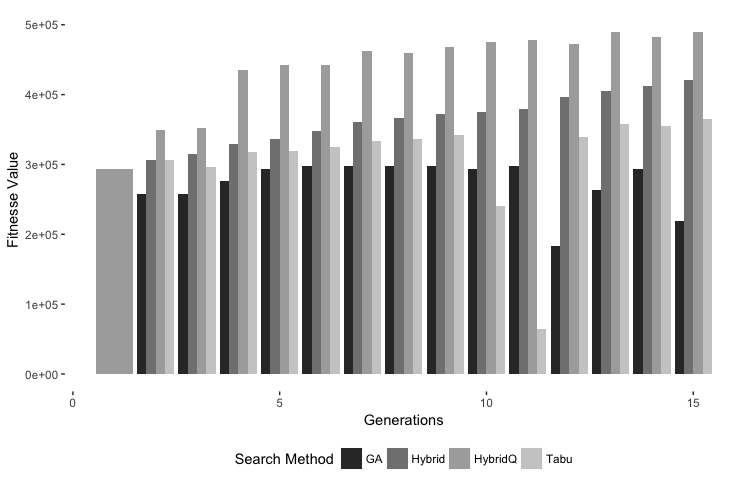
\includegraphics[width=0.7\textwidth]{./images/experiment1-1.png}
\caption{fitness value obtained by Search Method }
\label{fig:fitnessbygeneration1}
\end{figure}




Despite having obtained the best fitness value in each generation, the Hybrid algorithm performs twice as many requests as the  tabu search (Fig. \ref{fig:numberofrequestsbysearchmethod}). The HybridQ algorithm obtained the best fitness value The Fig. \ref{fig:boxplot1} shows the average, minimal e maximum value by search method.


\begin{figure}[H]

\centering
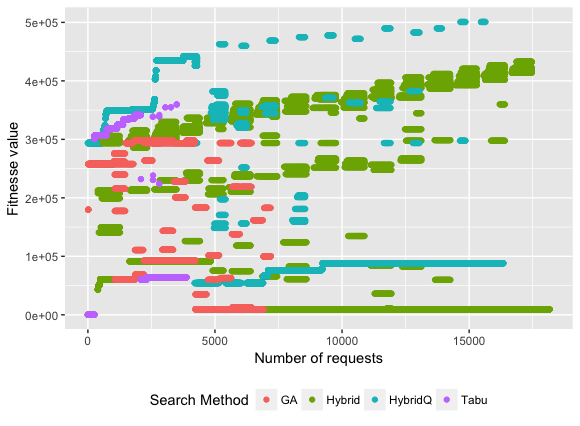
\includegraphics[width=0.8\textwidth]{./images/experiment1-3.png}
\caption{Number of requests by Search Method}
\label{fig:numberofrequestsbysearchmethod}
\end{figure}
\begin{figure}[H]
\centering
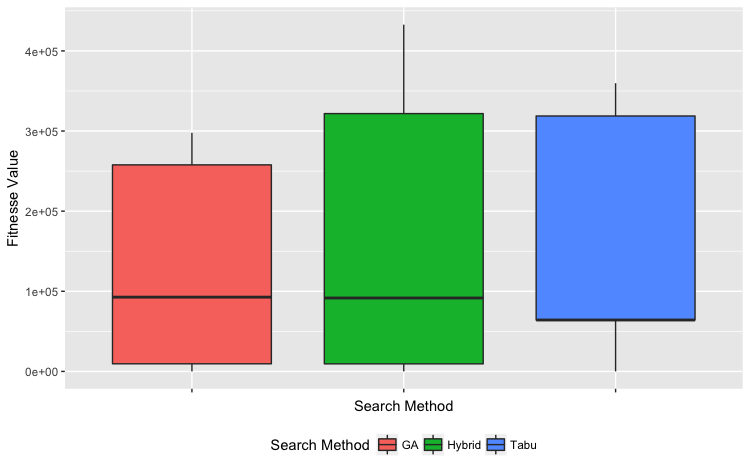
\includegraphics[width=0.8\textwidth]{./images/experiment1-4.png}
\caption{Average, median, maximum and minimal fitness value by Search Method}
\label{fig:boxplot1}

\end{figure}

The Fig. \ref{fig:summaryboxplot1} presents the maximum, average, median and minimum fitness value by generation. The maximun fitness value increases at each generation. The Fig. \ref{fig:density1} presents the density graph of number of users by fitness value. The range between 100 and 150 users has the highest number of individuals found with higher fitness value.

\begin{figure}[H]

\centering
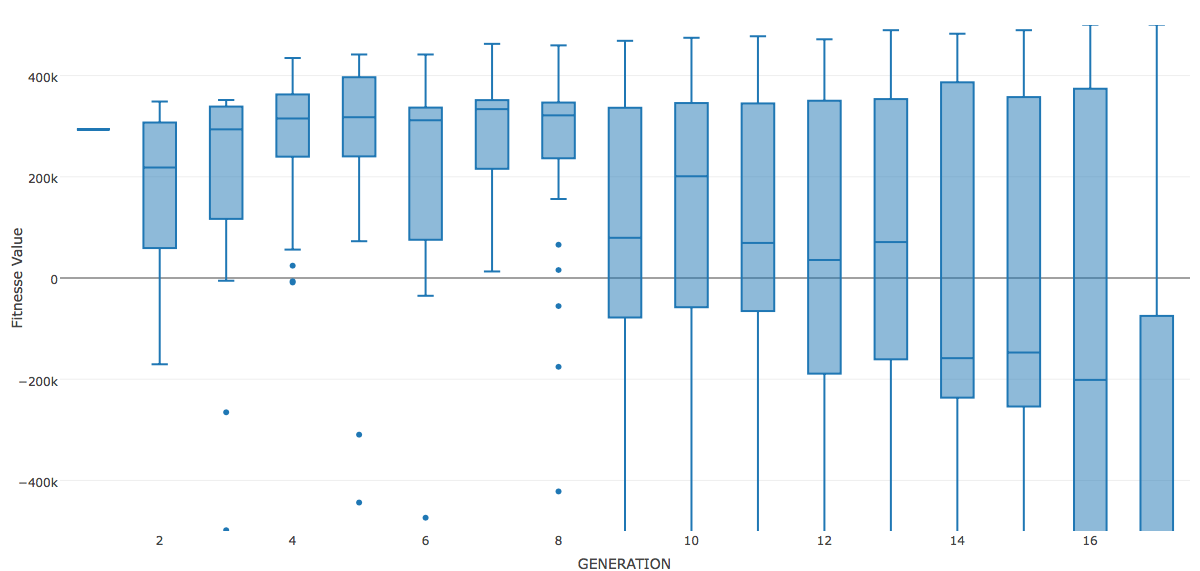
\includegraphics[width=1\textwidth]{./images/experiment1-5.png}
\caption{fitness value by generation}
\label{fig:summaryboxplot1}
\end{figure}
\begin{figure}[H]
\centering
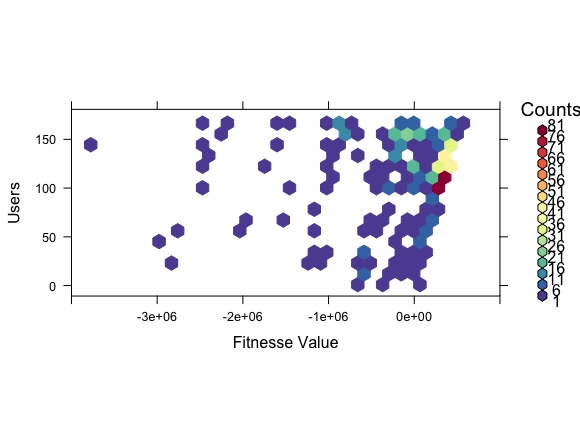
\includegraphics[width=1\textwidth]{./images/experiment1-6.png}
\caption{Density graph of number of users by fitness value}
\label{fig:density1}

\end{figure}

Table \ref{tab:bestindividuals} shows 4 individuals with 164 to 169 users. These are the scenarios with the maximum number of users found with the best response time. The first individual has 153 users on Happy Scenario 2, 16 users on Happy Scenario 1 and a response time of 13 seconds. None of the best individuals has one of the antipatterns used in the experiment.



% Please add the following required packages to your document preamble:
% \usepackage[table,xcdraw]{xcolor}
% If you use beamer only pass "xcolor=table" option, i.e. \documentclass[xcolor=table]{beamer}
\begin{table}[h]
\centering
\caption{Best individuals found in the first experiment}
\label{tab:bestindividuals}
\begin{tabular}{lllllll}
\rowcolor[HTML]{C0C0C0} 
\textbf{Search Method} & \textbf{Generation} & \textbf{Users} & \textbf{fitness Value} & \textbf{Happy 2} & \textbf{Happy 1} & \textbf{Resp. Time} \\
HybridQ & 17 & 169 & 500740 & 153 & 16 & 13 \\
HybridQ & 16 & 169 & 500700 & 153 & 16 & 15 \\
HybridQ & 13 & 164 & 489740 & 149 & 15 & 13 \\
HybridQ & 15 & 164 & 489740 & 149 & 15 & 13
\end{tabular}
\end{table}

Fig. \ref{fig:responsetimegenerationalltests1} presents the response time by number of users of individuals with Happy Scenario 1 and Happy Scenario 2. The Figure illustrates that the individuals with best fitness value has more users and minor response time. The Fig. \ref{fig:fitnessgenerationalltests1-1} presents the response time by number of users of individuals with the Ramp and Circuitous Treasure antipatterns scenarios. The Figure illustrates the smallest number of individuals with the antipatterns when compared to individuals who use the happy scenarios.


\begin{figure}[H]
\centering
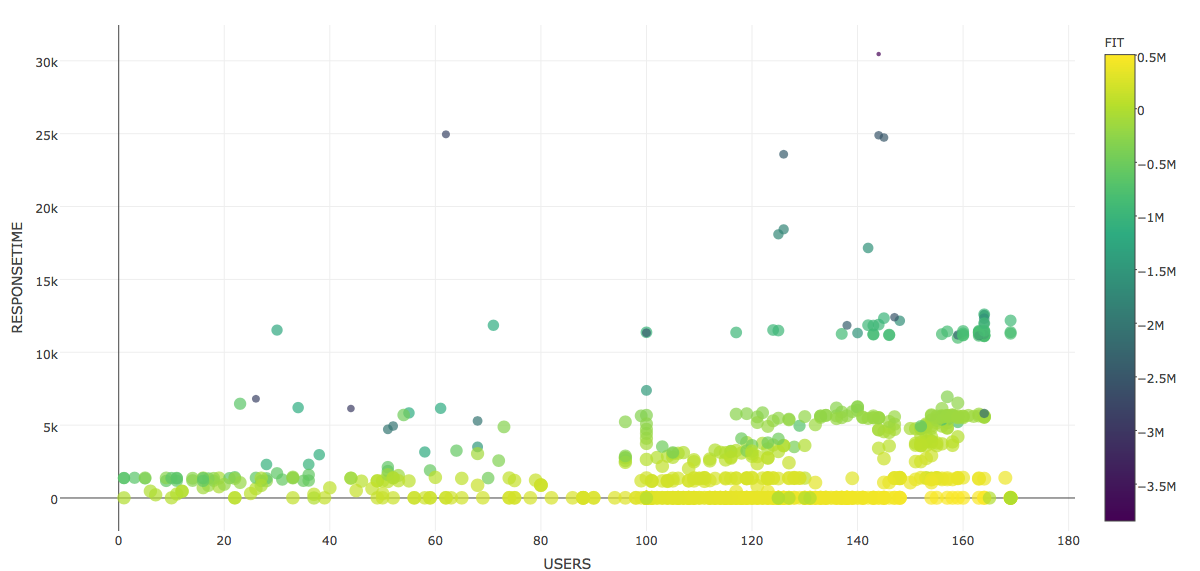
\includegraphics[width=1\textwidth]{./images/experiment1-7.png}
\caption{Response time by number of users of individuals with Happy Scenario 1 and Happy Scenario 2}
\label{fig:responsetimegenerationalltests1}
\end{figure}


\begin{figure}[H]
\centering
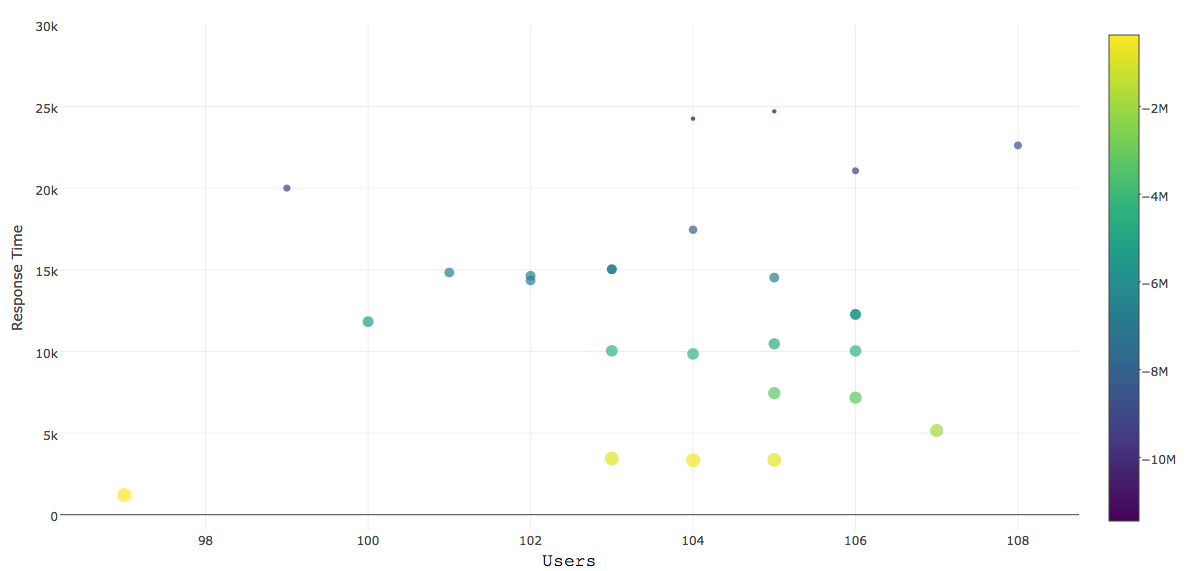
\includegraphics[width=1\textwidth]{./images/experiment1-8.png}
\caption{Response time by number of users of individuals with the Ramp and Circuitous Treasure antipatterns}
\label{fig:fitnessgenerationalltests1-1}

\end{figure}

Fig. \ref{fig:mdpexperiment1} presents the markov decision process for the experiment. When the response time it is bellow or equal the service level, the action with major reward it is increase the number of users and include more positions with the Happy Scenario 2 (Happy 2). When the response time is above the service level, the action with major reward value it is decrease the number of users and include more positions with the Happy Scenario 2. The actions  with minor value of reward contais the both antipatterns Circuitous Treasure (CTH) and The Ramp antipatterns (Ramp).

In the first experiment, We conclude that the metaheuristics converged to scenarios with an happy path, excluding the scenarios with antipatterns. The hybridQ and hybrid metaheuristic returned individuals with higher fitness scores. However, the Hybrid metaheuristic made twice as many requests than Tabu Search to overcome it. 

\begin{figure}[h]
\centering
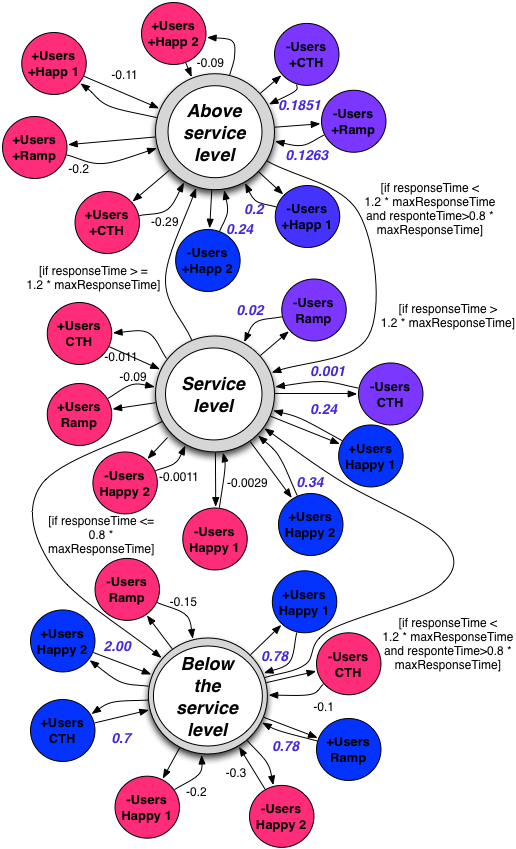
\includegraphics[width=0.6\textwidth]{./images/mdpexperiment.png}
\caption{Markov decision process of experiment with Circuitous Treasure and The Ramp antipatterns}
\label{fig:mdpexperiment1}

\end{figure}

\FloatBarrier
\subsection{The Tower Babel  and Unbalanced Processing experiment}

The experiment was carried out for 6 continuous hours. All tests in the experiment were conducted without the need of a tester. In this experiment, Scenarios were generated with Tower Babel and Unbalanced Processing antipattern as well as scenarios with Happy Scenario 1, Happy Scenario 2 and mixed scenarios. The Fig. \ref{fig:fitnessbygeneration2}  presents the fitness value obtained by each metaheuristic. The SA algorithm obtained the worst fitness values. Hybrid metaheuristic obtained the better fitness values.


\begin{figure}[h]
\centering
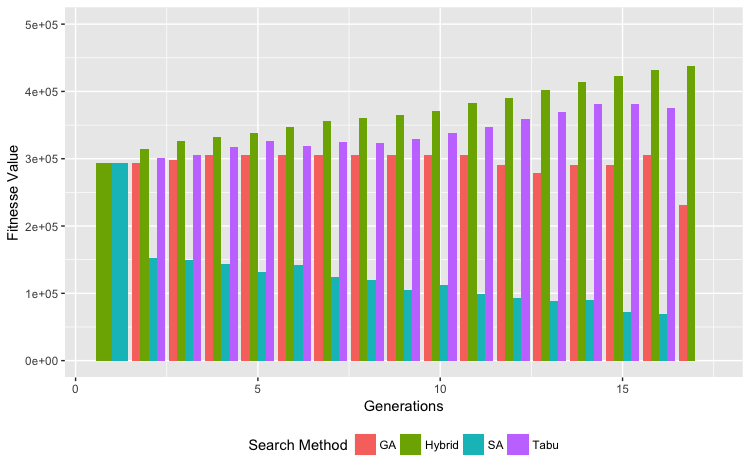
\includegraphics[width=.9\textwidth]{./images/experiment2-7.png}
\caption{Fitness value obtained by Search Method}
\label{fig:fitnessbygeneration2}
\end{figure}

As in the first experiment, the Hybrid algorithm performs twice as many requests as the second one, the tabu search (Fig. \ref{fig:numberofrequestsbysearchmethod2}). The Fig. \ref{fig:boxplot2} shows the average, minimal e maximum value by search method. The Fig. \ref{fig:summaryboxplot2} presents the maximum, average, median and minimum fitness value by generation. The maximun fitness value increases at each generation. The Fig. \ref{fig:density2} presents the density graph of number of users by fitness value. The range between 100 and 150 users has the highest number of individuals found with higher fitness value.


\begin{figure}[h]
\begin{minipage}{.5\textwidth}
\centering
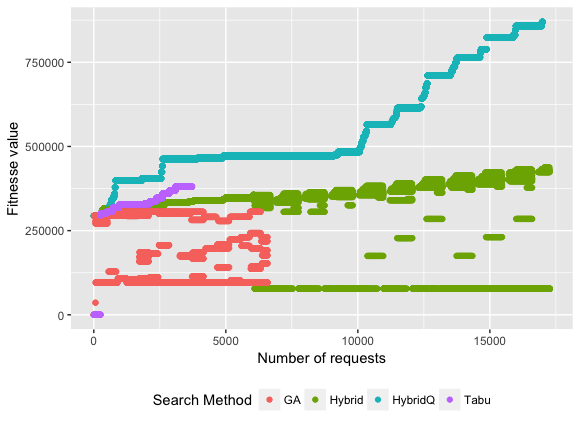
\includegraphics[width=1\textwidth]{./images/experiment2-1.png}
\caption{Number of requests by Search Method}
\label{fig:numberofrequestsbysearchmethod2}
\end{minipage}
\begin{minipage}{.5\textwidth}
\centering
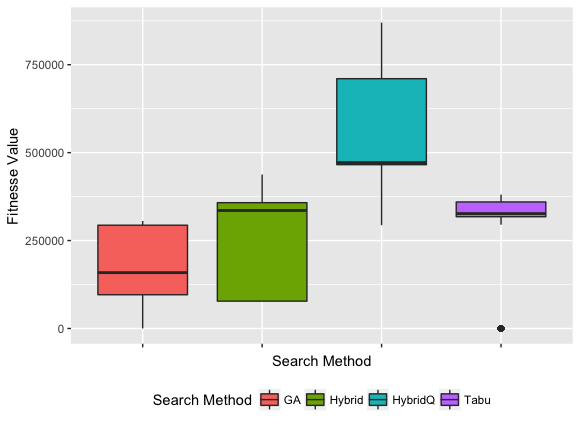
\includegraphics[width=1\textwidth]{./images/experiment2-2.png}
\caption{Fitness value by generation in all tests}
\label{fig:boxplot2}
\end{minipage}

\end{figure}



\begin{figure}[h]
\begin{minipage}{.5\textwidth}
\centering
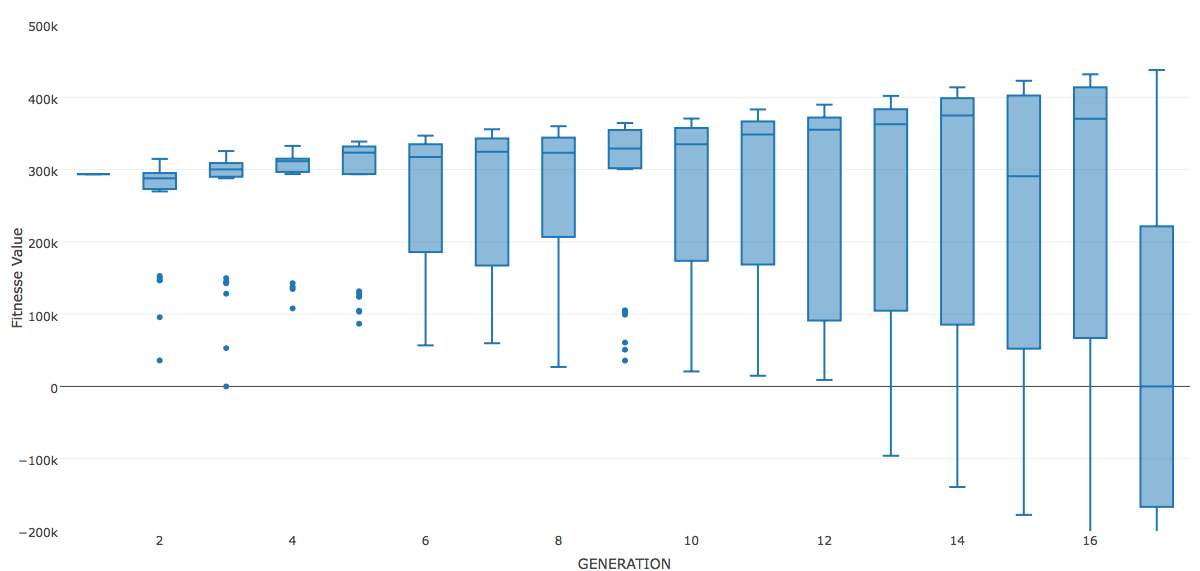
\includegraphics[width=1\textwidth]{./images/experiment2-3.png}
    \caption{Response time by generation in all tests scenarios}
\label{fig:summaryboxplot2}
\end{minipage}
\begin{minipage}{.5\textwidth}
\centering
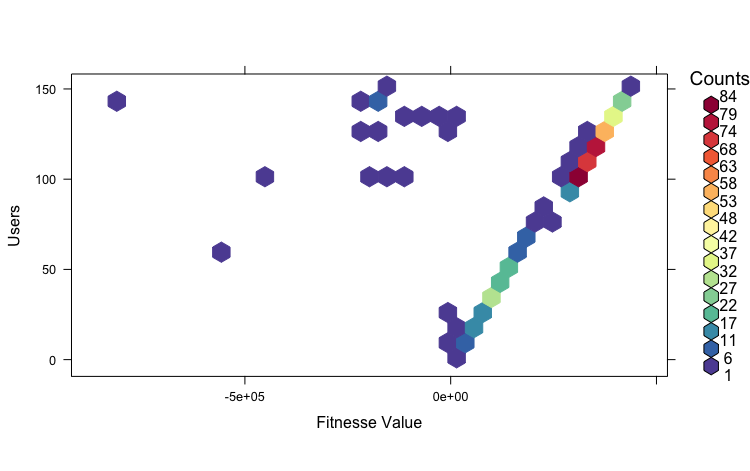
\includegraphics[width=1\textwidth]{./images/experiment2-4.png}
\caption{Finesse value by generation in all tests}
\label{fig:density2}
\end{minipage}

\end{figure}

Table \ref{tab:bestindividuals2} shows 4 individuals with 279 to 292 users.  The first individual has 121 users on Happy Scenario 2, 171 users on Happy Scenario 1 and a response time of 11 seconds. None of the best individuals found implements the Unbalanced Processing or Tower Babel antipattern.

Fig. \ref{fig:responsetimegenerationalltests2} presents the response time by number of users of individuals with Happy Scenario 1 and Happy Scenario 2. The Figure illustrates that the individuals with best fitness value has more users and minor response time. The Fig. \ref{fig:fitnessgenerationalltests2-1} presents the response time by number of users of individuals with with Unbalanced Processing and Tower Babel antipatterns scenarios. The Figure illustrates the smallest number of individuals with the  Unbalanced Processing and Tower Babel antipattern when compared to individuals who use the happy scenarios and the Tower Babel antipattern.



\begin{figure}[h]
\centering
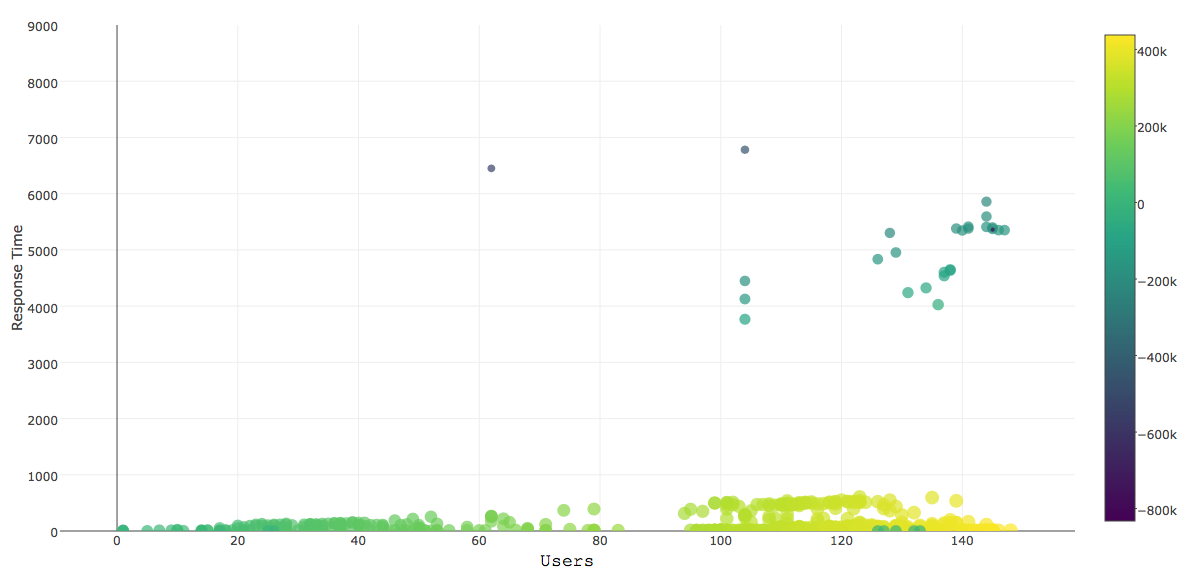
\includegraphics[width=1\textwidth]{./images/experiment2-5.png}
\caption{Response time by number of users of individuals with Happy Scenario 1, Happy Scenario 2 and Tower Babel antipattern}
\label{fig:responsetimegenerationalltests2}
\end{figure}


\begin{figure}[h]
\centering
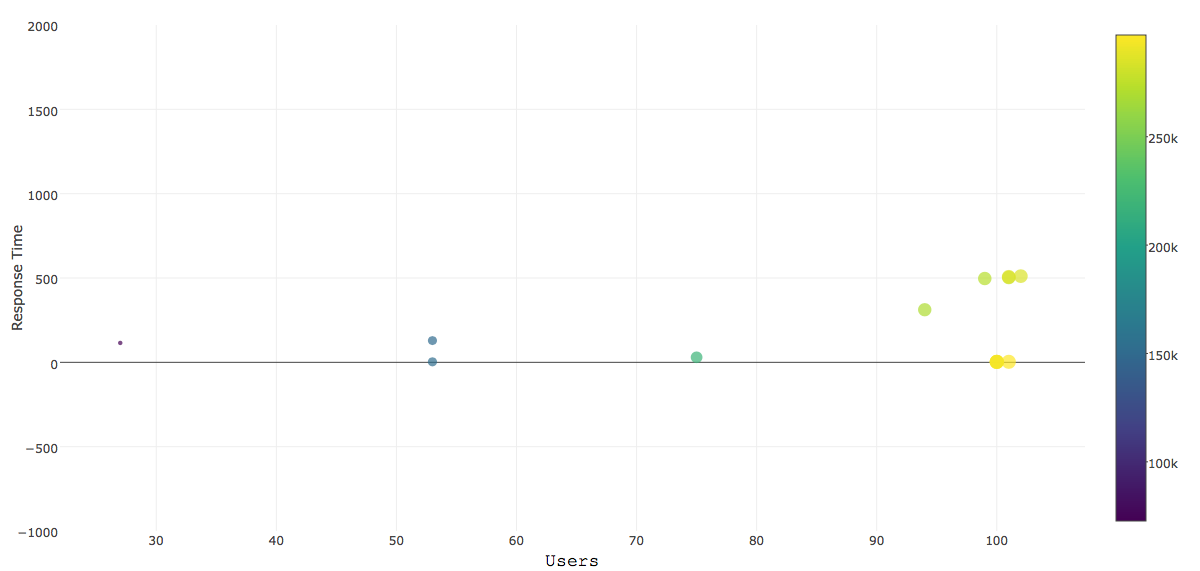
\includegraphics[width=1\textwidth]{./images/experiment2-6.png}
\caption{Response time by number of users of individuals with Unbalanced Processing antipattern}
\label{fig:fitnessgenerationalltests2-1}
\end{figure}


We conclude that the metaheuristics converged to scenarios with an happy path, excluding the scenarios with Unbalanced Processing and Tower Babel antipattern. The hybrid metaheuristic with Q-Learning (HybridQ) returned individuals with higher fitness scores. The Hybrid metaheuristic (Hybrid) made twice as many requests than Tabu Search to overcome it. The SA algorithm obtained the worst fitness values. The algorithm initially used a scenario with an antipattern and found neighbors that still using an antipattern over the 17 generations of the experiment. The individual with best fitness value has 121 users on Happy Scenario 2, 171 users on Happy Scenario 1 and a response time of 11 seconds.

% Please add the following required packages to your document preamble:
% \usepackage[table,xcdraw]{xcolor}
% If you use beamer only pass "xcolor=table" option, i.e. \documentclass[xcolor=table]{beamer}
\begin{table}[h]
\centering
\caption{Best individuals found in the second experiment}
\label{tab:bestindividuals2}
\begin{tabular}{lllllll}
\rowcolor[HTML]{FFCCC9} 
\textbf{Search Method} & \textbf{Generation} & \textbf{Users} & \textbf{fitness Value} & \textbf{Happy 2} & \textbf{Happy 1} & \textbf{Time} \\ 
\multicolumn{1}{l}{HybridQ} & \multicolumn{1}{l}{17} & \multicolumn{1}{l}{292} & \multicolumn{1}{l}{869780}  & \multicolumn{1}{l}{121} & \multicolumn{1}{l}{171} & \multicolumn{1}{l}{11} \\ 
\multicolumn{1}{l}{HybridQ} & \multicolumn{1}{l}{16} & \multicolumn{1}{l}{288} & \multicolumn{1}{l}{857780} &  \multicolumn{1}{l}{103} & \multicolumn{1}{l}{185} & \multicolumn{1}{l}{11} \\ 
\multicolumn{1}{l}{HybridQ} & \multicolumn{1}{l}{16} & \multicolumn{1}{l}{284} & \multicolumn{1}{l}{845880} &  \multicolumn{1}{l}{167} & \multicolumn{1}{l}{117} & \multicolumn{1}{l}{10} \\ 
\multicolumn{1}{l}{HybridQ} & \multicolumn{1}{l}{16} & \multicolumn{1}{l}{279} & \multicolumn{1}{l}{830780} &  \multicolumn{1}{l}{144} & \multicolumn{1}{l}{135} & \multicolumn{1}{l}{11} \\ 
\end{tabular}
\end{table}

\section{Moodle Application Experiment}

This experiment used a Moodle application installed in a machine with 500 GB of hard disk space and 8 GB of memory. The study used six application scenarios:

\begin{itemize}
\item PostDeleteMessage: This scenario posts and deletes messages in the Moodle application.
\item MyHome: This scenario accesses the homepage of the user's application.
\item Login: This scenario is responsible for user authentication by the application.
\item Notifications: This scenario involves entering the notification page of each user.
\item Start Page: This scenario shows the initial start page of the application.
\item Badge: This scenario involves entering the badge page.
\end{itemize}

The experiment used the following fitness function:

\begin{equation}
\begin{aligned}
fitness=0.9* 90percentiletime\\
+0.1*80percentiletime\\+
0.1*70percentiletime+\\
0.1*maxResponseTime+\\
0.2*numberOfUsers-penalty
\end{aligned}
\end{equation}

The maximum tolerated response time in the test was 30 seconds.  Any  individuals who obtained a time longer than the stipulated maximum time suffered penalties.  The whole process of stress and performance tests, which took 3 days and about 1800 executions, was carried out without the need for monitoring by a test designer. The tool automatically selected the next scenarios to be run up to the limit of six generations previously established. 

Table \ref{tab:secondexperiment} presents the maximum fitness value obtained by the hybrid metaheuristic (HM) approach, genetic algorithm (GA), simulated annealing (SA), and Tabu search (TS) in each generation. 


\begin{table}[h]
\centering
\caption{Results obtained from the second experiment}
\label{tab:secondexperiment}
\begin{tabular}{|l|l|l|l|l|}
\hline
GEN & HM    & TS    & GA    & SA    \\
\hline
1          & 32242 & 32242 & 32242 & 32242 \\
\hline
2          & 34599 & 32443 & 26290 & 35635 \\
\hline
3          & 35800 & 34896 & 34584 & 34248 \\
\hline
4          & 35782 & 34912 & 32689 & 25753 \\
\hline
5          & 35611 & 31833 & 34631 & 8366  \\
\hline
6          & 35362 & 35041 & 33397 & 9706 \\
\hline
\end{tabular}
\end{table}


The small number of samples of the experiment is insufficient to give a statistical significance to the results of the Wilcoxon procedure. However, it is noted that, in four of six generations, the collaborative approach presented the best values. The experiment succeeded in finding 29 individuals whose maximum time expected by the application was obtained.  Table \ref{tab:secondexperiment1} shows an example of the six individuals with the highest fitness values in the second experiment. The table shows the fitness value (Fit);  the name of the scenario (Scenario); the number of users (Users); and the percentiles of 90\%, 80\%, and 70\% (90per, 80per and 70per) in seconds.  

% Please add the following required packages to your document preamble:
% \usepackage{multirow}
\begin{table}[h]
\centering
\caption{Example of individuals obtained in the second experiment}
\label{tab:secondexperiment1}
\begin{tabular}{|p{0.2cm}|l|l|l|p{1.00cm}|p{1.00cm}|p{1.00cm}|}
\hline
Id&Fit&Scenario&Users&90per&80per&70per\\ \hline
\multirow{2}{*}{1} & \multirow{2}{*}{35800} & MyHome        & 31              & \multirow{2}{*}{30} & \multirow{2}{*}{29} & \multirow{2}{*}{10} \\ \cline{3-4}
                   &                        & Badges        & 4               &                     &                     &                     \\ \hline
\multirow{3}{*}{2} & \multirow{3}{*}{35795} & MyHome        & 30              & \multirow{3}{*}{30} & \multirow{3}{*}{29} & \multirow{3}{*}{10} \\ \cline{3-4}
                   &                        & Notifications & 2               &                     &                     &                     \\ \cline{3-4}
                   &                        & Badges        & 2               &                     &                     &                     \\ \hline
\multirow{2}{*}{3} & \multirow{2}{*}{35782} & MyHome        & 32              & \multirow{2}{*}{30} & \multirow{2}{*}{29} & \multirow{2}{*}{10} \\ \cline{3-4}
                   &                        & Badges        & 3               &                     &                     &                     \\ \hline
\multirow{3}{*}{4} & \multirow{3}{*}{35773} & MyHome        & 22              & \multirow{3}{*}{30} & \multirow{3}{*}{29} & \multirow{3}{*}{10} \\ \cline{3-4}
                   &                        & Notifications & 6               &                     &                     &                     \\ \cline{3-4}
                   &                        & Badges        & 9               &                     &                     &                     \\ \hline
\multirow{2}{*}{5} & \multirow{2}{*}{35771} & MyHome        & 28              & \multirow{2}{*}{30} & \multirow{2}{*}{29} & \multirow{2}{*}{9}  \\ \cline{3-4}
                   &                        & Badges        & 6               &                     &                     &                     \\ \hline
\multirow{2}{*}{6} & \multirow{2}{*}{35683} & MyHome        & 27              & \multirow{2}{*}{30} & \multirow{2}{*}{29} & \multirow{2}{*}{8}  \\ \cline{3-4}
                   &                        & Badges        & 10              &                     &                     &                     \\ \hline
\end{tabular}
\end{table}


Table \ref{fig:gened} presents the percentage of genes in all test scenarios by generation with and without collaboration. Most of the genes converged to the MyHome feature, which had the highest application response time.


% Please add the following required packages to your document preamble:
% \usepackage[table,xcdraw]{xcolor}
% If you use beamer only pass "xcolor=table" option, i.e. \documentclass[xcolor=table]{beamer}
\begin{table}[h!]
\centering
\caption{Percentage of genes in each scenario by generation }
\label{fig:gened}
\begin{tabular}{c|c|c|c|c|c|c|c|}
\hline
\rowcolor[HTML]{D3D3D3} 
\multicolumn{1}{|c|}{\cellcolor[HTML]{FFFFFF}\textbf{Gen/}}   & \multicolumn{7}{c|}{\cellcolor[HTML]{D3D3D3}\textbf{Non collaboration approach}}                                                                                                                                                       \\ \cline{2-8} 
\multicolumn{1}{|c|}{\textbf{Scenarios}}                      & \cellcolor[HTML]{F8FF00}Initial & \cellcolor[HTML]{F8FF00}1 & \cellcolor[HTML]{F8FF00}2 & \cellcolor[HTML]{F8FF00}3 & \cellcolor[HTML]{F8FF00}4 & \cellcolor[HTML]{F8FF00}5 & \cellcolor[HTML]{F8FF00}6                                \\ \hline
\multicolumn{1}{|c|}{\cellcolor[HTML]{D3D3D3}Badges}          & 20                              & 18                        & 16                        & 24                        & 15                        & 16                        & 17                                                       \\ \hline
\rowcolor[HTML]{F8FF00} 
\multicolumn{1}{|c|}{\cellcolor[HTML]{F8FF00}\textbf{MyHome}} & \textbf{15}                     & \textbf{59}               & \textbf{55}               & \textbf{48}               & \textbf{53}               & \textbf{50}               & \multicolumn{1}{l|}{\cellcolor[HTML]{F8FF00}\textbf{52}} \\ \hline
\multicolumn{1}{|c|}{\cellcolor[HTML]{D3D3D3}StartPage}       & 15                              & 10                        & 12                        & 11                        & 20                        & 18                        & \multicolumn{1}{l|}{19}                                  \\ \hline
\multicolumn{1}{|c|}{\cellcolor[HTML]{D3D3D3}Notifications}   & 25                              & 5                         & 11                        & 10                        & 9                         & 10                        & \multicolumn{1}{l|}{9}                                   \\ \hline
\multicolumn{1}{|c|}{\cellcolor[HTML]{D3D3D3}Post}            & 8                               & 3                         & 1                         & 3                         & 1                         & 2                         & \multicolumn{1}{l|}{1}                                   \\ \hline
\multicolumn{1}{|c|}{\cellcolor[HTML]{D3D3D3}Login}           & 17                              & 5                         & 5                         & 4                         & 2                         & 4                         & \multicolumn{1}{l|}{2}                                   \\ \hline
\multicolumn{1}{l|}{}                                         & \multicolumn{7}{c|}{\cellcolor[HTML]{D3D3D3}\textbf{Collaboration approach}}                                                                                                                                                           \\ \hline
\multicolumn{1}{|c|}{\cellcolor[HTML]{D3D3D3}Badges}          & 20                              & 29                        & 16                        & 25                        & 9                         & 16                        & 9                                                        \\ \hline
\rowcolor[HTML]{F8FF00} 
\multicolumn{1}{|c|}{\cellcolor[HTML]{F8FF00}\textbf{MyHome}} & \textbf{15}                     & \textbf{29}               & \textbf{69}               & \textbf{49}               & \textbf{74}               & \textbf{66}               & \textbf{76}                                              \\ \hline
\multicolumn{1}{|c|}{\cellcolor[HTML]{D3D3D3}StartPage}       & 15                              & 22                        & 10                        & 21                        & 10                        & 10                        & 8                                                        \\ \hline
\multicolumn{1}{|c|}{\cellcolor[HTML]{D3D3D3}Nofications}     & 25                              & 10                        & 1                         & 1                         & 2                         & 1                         & 3                                                        \\ \hline
\multicolumn{1}{|c|}{\cellcolor[HTML]{D3D3D3}Post}            & 8                               & 2                         & 1                         & 1                         & 1                         & 2                         & 1                                                        \\ \hline
\multicolumn{1}{|c|}{\cellcolor[HTML]{D3D3D3}Login}           & 17                              & 8                         & 3                         & 3                         & 4                         & 5                         & 3                                                        \\ \hline
\end{tabular}
\end{table}


%\begin{figure}[h]
%\centering
%\caption{Percentage of genes in all test scenarios by generation }
%\includegraphics[width=0.5\textwidth]{./images/gened.png}
%\label{fig:gened}
%\end{figure}

\section{JPetStore Application Experiments}

One experiment was conducted to test the use of the HybridQ algorithm in a real implemented application. The chosen application was the JPetStore, available at \url{https://hub.docker.com/r/pocking/jpetstore/}. The maximum tolerated response time in the test was 500 seconds.  Any  individuals who obtained a time longer than the stipulated maximum time suffered penalties.  The whole process of stress and performance tests, which run for 2 days and  with about 1.800 executions, was carried out without the need for monitoring by a test designer. The tool automatically selected the next scenarios to be run up to the limit of eleven generations previously established. The experiments use the follow application features:


\begin{itemize}
\item Enter in the Catalog: the application presents the catalog of pets.
\item Fish: The application shows the recorded fish items.
\item Register:  a new user is registered into the system.
\item Dogs: The application shows the recorded dogs supplies.
\item Shopping Cart: the application displays the shopping cart.
\item Add or Remove in Shopping Cart: the application adds and removes items from shopping cart.
\end{itemize}

Table \ref{tab:isolated} presents the maximum number of users found in each scenario who obtained a time lower than the stipulated maximum time of 500 seconds.


% Please add the following required packages to your document preamble:
% \usepackage[table,xcdraw]{xcolor}
% If you use beamer only pass "xcolor=table" option, i.e. \documentclass[xcolor=table]{beamer}
\begin{table}[h!]
\centering
\caption{Maximum number of users of isolated test scenarios }
\label{tab:isolated}
\begin{tabular}{ll}
\rowcolor[HTML]{FFCCC9} 
\textbf{Scenario}    & \textbf{Max number of Users} \\
Fish                 & 85                           \\
Enter in The Catalog & 60                           \\
Dogs                 & 75                           \\
Cart                 & 70                           \\
Register             & 90                          
\end{tabular}
\end{table}

The Fig. \ref{fig:surface} and \ref{fig:surface2} present the response time by generation and by the number of users.


\begin{figure}[h]
\begin{minipage}{.5\textwidth}
\centering
\includegraphics[width=1\textwidth]{./images/SearchSurface.png}
\caption{Search space of individuals found in the experiment by search method}
\label{fig:surface}
\end{minipage}
\begin{minipage}{.5\textwidth}
\centering
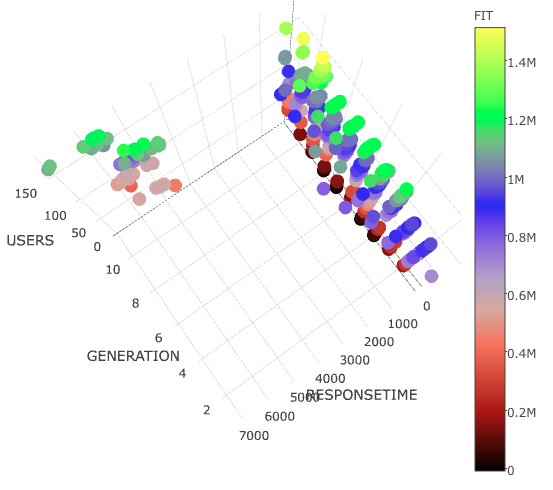
\includegraphics[width=1\textwidth]{./images/searchsurface2.png}
\caption{Search space of individuals found in the experiment by fitness value}
\label{fig:surface2}
\end{minipage}
\end{figure}

The experiment used the following fitness function:

\begin{equation}
\begin{aligned}
fitness=\begin{cases} n*\{3000*numberOfUsers-20* 90percentiletime-20*80percentiletime\\-20*70percentiletime
-20*maxResponseTime-penalty\} , \textsf{where n is the }\\\ \textsf{ number of features used by the test in a set of previous selected application} \\ \textsf{features}
\end{cases}
\end{aligned}
\end{equation}


The purpose of the fitness function is to maximize the number of users and minimize the response time in the tests containing a selected \textit{n} functionalities. For example, it is possible double the fitness value for tests that have the fish and user registration scenario. 

This experiment tries to find the scenarios with maximal number of users and best response time tests that contains the Cart and Register features. The Fig. \ref{fig:experiment31} and \ref{fig:experiment32} show the fitness value by generation. The HybridQ obtained the best fitness values in all generations.

\begin{figure}[h]
\begin{minipage}{.5\textwidth}
\centering
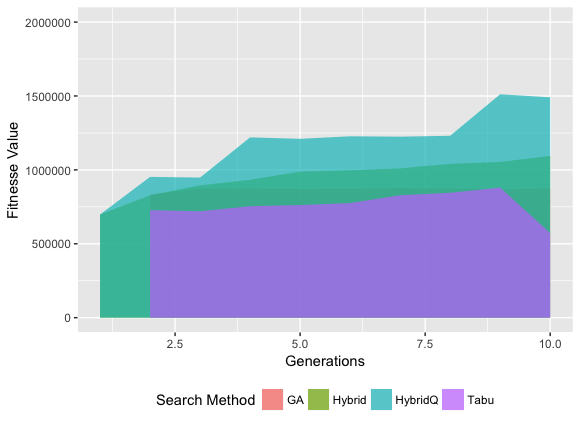
\includegraphics[width=1\textwidth]{./images/experiment3-1.png}
\caption{Fitness value by generation on JPetStore First experiment}
\label{fig:experiment31}
\end{minipage}
\begin{minipage}{.5\textwidth}
\centering
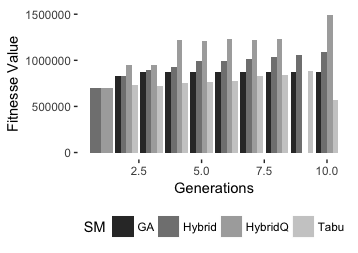
\includegraphics[width=1\textwidth]{./images/experiment3-2.png}
\caption{Fitness value by generation on JPetStore First experiment}
\label{fig:experiment32}
\end{minipage}
\end{figure}

The Fig. \ref{fig:numberofrequestsbysearchmethod3} shows the fitness value by number of request by each Search Method. In the Figure, it is possible to observe that HybridQ obtained the best fitness value to same number of requests of the other algorithms.

\begin{figure}[h]
\begin{minipage}{.5\textwidth}
\centering
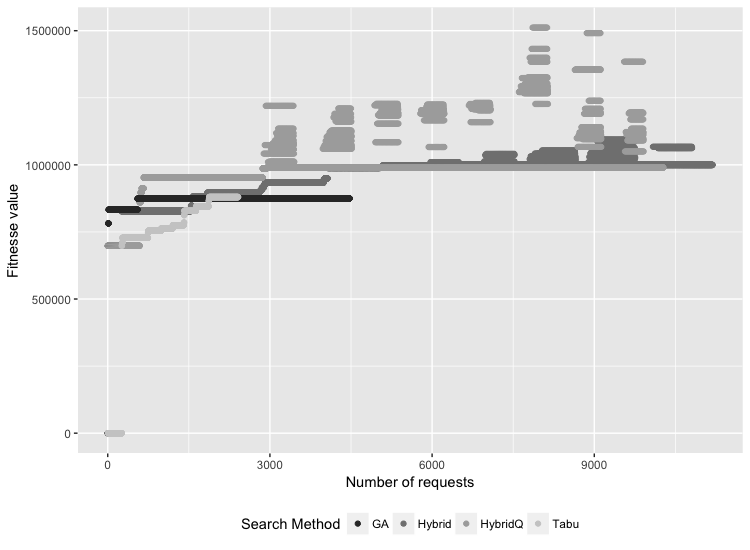
\includegraphics[width=1\textwidth]{./images/experiment3-3.png}
\caption{Number of requests by Search Method}
\label{fig:numberofrequestsbysearchmethod3}
\end{minipage}
\begin{minipage}{.5\textwidth}
\centering
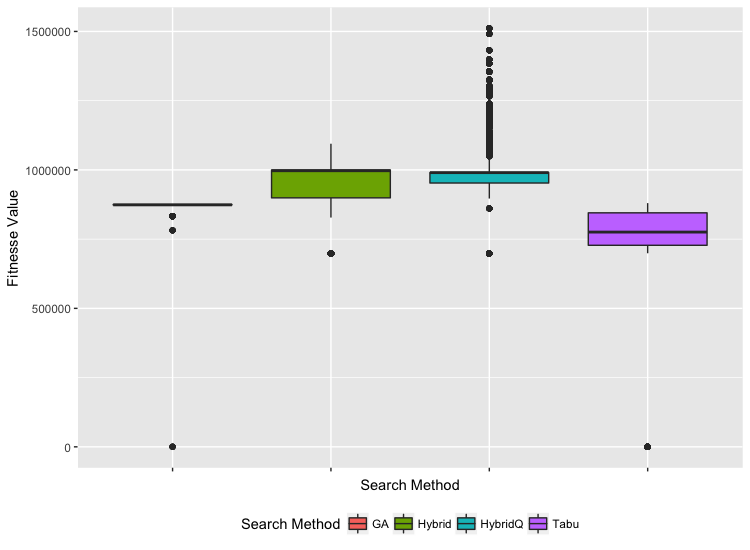
\includegraphics[width=1\textwidth]{./images/experiment3-4.png}
\caption{Fitness value by generation in all tests}
\label{fig:boxplot3}
\end{minipage}

\end{figure}

Table \ref{tab:bestindividuals3} shows 4 individuals with 233 to 398 users.  The first individual has 73 users on fish scenario, 17 users on Dogs scenario, 50 users on Cart scenario, 33 Users on register scenario  and a response time of 357 seconds. 

% Please add the following required packages to your document preamble:
% \usepackage[table,xcdraw]{xcolor}
% If you use beamer only pass "xcolor=table" option, i.e. \documentclass[xcolor=table]{beamer}
\begin{table}[h!]
\centering
\caption{Best individuals found in JPetStore first experiment}
\label{tab:bestindividuals3}
\begin{tabular}{lllllllll}
\rowcolor[HTML]{C0C0C0} 
\textbf{Search Method} & \textbf{Response} & \textbf{Users} & \textbf{Gen} & \textbf{Fitness} & \textbf{fish} & \textbf{Dogs} & \textbf{Cart} & \textbf{Register} \\
HybridQ                & 357               & 173            & 9            & 44773            & 73             & 17            & 50            & 33                \\
HybridQ                & 398               & 171            & 10           & 44831            & 57             & 33            & 48            & 33                \\
HybridQ                & 331               & 164            & 9            & 44774            & 71             & 14            & 51            & 28                \\
HybridQ                & 233               & 159            & 9            & 44783            & 63             & 31            & 32            & 33               
\end{tabular}
\end{table}

We conclude that HybridQ found the individuals with major number of uses. The scenario with major number of users is the Fish search feature. The hybrid metaheuristic with Q-Learning (HybridQ) returned individuals with higher fitness scores.  The individual with best fitness value has 73 users on fish scenario, 17 users on Dogs scenario, 50 users on Cart scenario, 33 Users on register scenario  and a response time of 357 seconds. 


\section{Experimental Results}

In this section, We present the result of the experiment which we carried out to verify the multiobjective NSGA-II   implementation. The experiment was conducted to validate the use of NSGA-II multiobjective algorithm with a real implemented application. The chosen application was the JPetStore, available at \url{https://hub.docker.com/r/pocking/jpetstore/}. The maximum tolerated response time in the test was 500 seconds.  The whole process of stress  tests, which run for 3 days and 492 executions, was carried out without the need for monitoring by a test designer. The tool automatically selected the next scenarios to be run up to the limit of 123 generations previously established by algorithm. The experiments use the follow application features:


\begin{itemize}
\item Enter in the Catalog: the application presents the catalog of pets.
\item Fish: The application shows the recorded fish items.
\item Register:  a new user is registered into the system.
\item Dogs: The application shows the recorded dogs supplies.
\item Shopping Cart: the application displays the shopping cart.
\item Add or Remove in Shopping Cart: the application adds and removes items from shopping cart.
\end{itemize}

The experiments used an initial population of 4 individuals by metaheuristic. The genetic algorithm used the top 10 individuals from each generation in the crossover operation  The mutation operation was applied to 10\% of the population on each generation. The objective functions applied is intended to minimize the number of users and maximize the response time of the scenarios being tested. A penalty is applied when an application under test takes a longer time to respond than the maximum response time expected. 

The experiment used the following objective equations:

\begin{equation}
\begin{aligned}
objective function 1 =-3*numberOfUsers\\
-penalty\\
\end{aligned}
\end{equation}


\begin{equation}
\begin{aligned}
objective function 2 =responsetime\\
-penalty\\
\end{aligned}
\end{equation}

The first objective function seeks to find workloads with greater number of users and shorter response time. The second objective function seeks to find workloads with fewer users and longer response times. The penalty is calculated by the follow equation:

\begin{equation}
\begin{aligned}
penalty=100 * \Delta \\
\Delta=(t_{Current Response Time} - t_{Maximum Response Time Expected})\\
\end{aligned}
\end{equation}



\subsection{Experiment Research Questions}

The following research question is addressed:
\begin{itemize}
\item Does the NSGA-II algorithm find relevant workload scenarios according to the two test objectives?
\end{itemize}

\subsection{Variables}

The independent variable is the NSGA-II algorithm used in the test. The dependent variables are: the optimal workload scenario found by the algorithm.

\subsection{Hypotheses}

\begin{itemize}
\item With regard to multi-objectives applied in the experiment:
\begin{itemize}
\item $H_{0}$ (A null hypothesis) :The NSGA-II doesn't found workloads that meet the two objective functions used in the experiment.
\item $H_{1}$  : The NSGA-II  algorithm found workloads that meet the two objective functions used in the experiment.
\end{itemize}
\end{itemize}

\subsection{Results}

Fig. \ref{fig:paretofrontier1} and Table \ref{tab:results} present the results obtained in the experiment. The experiment found 9 optimal workloads (Pareto Frontier) that present a lower number of users with high response times. The workload number 1 with a single user accessing the dog scenario presented the response time of 245 seconds.  The workload number 2 with a single user accessing the dog scenario, 7 users accessing the Enter Catalog feature and 3 users in register functionality presented the response time of 400 seconds.



\begin{figure}[h]
\centering
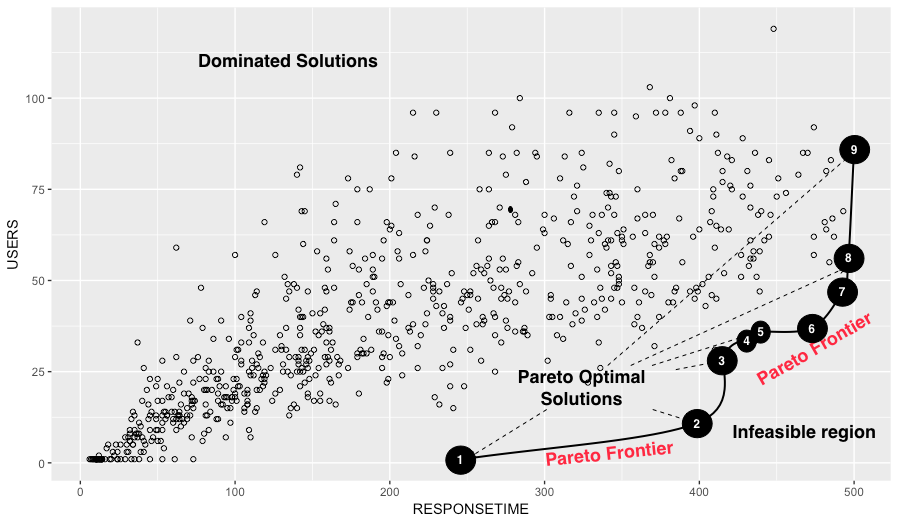
\includegraphics[width=1\textwidth]{./images/pareto0curve.png}
    \caption{Experiment Pareto Frontier}
\label{fig:paretofrontier1}
\end{figure}

% Please add the following required packages to your document preamble:
% \usepackage[table,xcdraw]{xcolor}
% If you use beamer only pass "xcolor=table" option, i.e. \documentclass[xcolor=table]{beamer}
\begin{table}[]
\centering
\caption{Pareto Frontier workloads results}
\label{tab:results}
\begin{tabular}{|l|l|l|l|l|l|l|l|l|}
\hline
\rowcolor[HTML]{C0C0C0} 
\textbf{N.} & \textbf{\begin{tabular}[c]{@{}l@{}}OBJ.\\ 1\end{tabular}} & \textbf{\begin{tabular}[c]{@{}l@{}}OBJ. \\ 2\end{tabular}} & \multicolumn{1}{c|}{\cellcolor[HTML]{C0C0C0}\textbf{\begin{tabular}[c]{@{}c@{}}Dogs\\ Users\end{tabular}}} & \textbf{\begin{tabular}[c]{@{}l@{}}Enter\\ Catalog\\ Users\end{tabular}} & \textbf{\begin{tabular}[c]{@{}l@{}}Fish\\ Users\end{tabular}} & \textbf{\begin{tabular}[c]{@{}l@{}}Register\\ Users\end{tabular}} & \textbf{\begin{tabular}[c]{@{}l@{}}Add\\ Rem.\\ Cart\end{tabular}} & \textbf{\begin{tabular}[c]{@{}l@{}}Cart\\ Users\end{tabular}} \\ \hline
\ding{202}           & -3                                                        & 245                                                        & 1                                                          &                                                                  &               &                   &                                                                    &               \\ \hline
\ding{203}           & -33                                                       & 400                                                        & 1                                                          & 7                                                                &               & 3                 &                                                                    &               \\ \hline
\ding{204}           & -87                                                       & 416                                                        & 5                                                          & 15                                                               & 4             & 5                 &                                                                    &               \\ \hline
\ding{205}          & -102                                                      & 434                                                        & 16                                                         & 17                                                               &               &                   &                                                                    & 1             \\ \hline
\ding{206}           & -105                                                      & 436                                                        & 15                                                         & 4                                                                & 8             & 3                 & 5                                                                  &               \\ \hline
\ding{207}           & -111                                                      & 472                                                        & 7                                                          & 13                                                               & 7             & 3                 & 7                                                                  &               \\ \hline
\ding{208}           & -141                                                      & 493                                                        & 7                                                          & 11                                                               & 11            & 7                 & 7                                                                  & 4             \\ \hline
\ding{209}           & -112                                                      & 496                                                        & 6                                                          &                                                                  & 12            & 8                 & 19                                                                 & 9             \\ \hline
\ding{210}           & -255                                                      & 499                                                        &                                                            & 54                                                               & 12            &                   & 7                                                                  & 12            \\ \hline
\end{tabular}
\end{table}


\subsection{Threats to validity}
\begin{itemize}
\item Construct Validity: 
In this work, we just evaluate the use of one multiobjective algorithm. However, several multiobjective algorithms could be applied.  There is still a reasonable distance between the Pareto frontier and the data obtained for the second objective, and more experiments are needed to validate the results.
\item Conclusion Validity: 
The workloads found by NSGA-II may be the result of the elitist strategy used in the algorithm that can be applied in the genetic algorithm.
\end{itemize}

